\epigraph{``Yes, it is easy to see that nearly six years of magical education has not been wasted on you ... Ghosts are transparent"}{Severus Snape}

Atmospheric dynamics is a core component of any computational model that is trying to simulate the atmosphere. It deals with motion in the atmosphere and its thermodynamic state\cite{the_what}. The ideal goals of studying this topic include: improving weather predictions, and understanding the implications of human-induced perturbations on the global climate\cite{why}. An example of a human-induced, or human-caused perturbation on the global climate would be the depletion of the ozone layer\cite{perturbation}. Another topical example of a human-induced perturbation would be the gradual heating of the planet through climate change. Advancements in the field of atmospheric dynamics has led to a dramatic decline in deaths from extreme weather phenomena, such as, hurricanes, tornadoes, and flash flooding\cite{deaths}.

\section{Development of the Idea}
I think it is extremely difficult to pinpoint exactly where the idea originated from; on reflection, however, the spark which really ignited the flame for this project came from a deep interest in the study of the atmosphere and by extension atmospheric science. I initially became interested in this topic based on two distinct factors. 

Initially, I became interested in the area of atmospheric science from watching a YouTuber named, Dr. Simon Clark. Dr. Simon Clark recently completed a PhD in theoretical atmospheric physics, researching dynamical stratosphere-troposphere coupling, and made a vlog series documenting his experiences. I was extremely intrigued by this series, with keen interest in his videos explaining his research. These videos captivated me and ultimately led me to reading his thesis (titled Quasi-geostrophic influence of the polar stratosphere on the troposphere)\cite{simonclark}.

Secondly, my interest also came from my concern over human caused climate change. I was extremely fascinated by how a gas, such as carbon dioxide, could capture so much more heat than oxygen, even though there is a higher concentration of oxygen in the atmosphere. This ultimately led to the original idea for this project: creating a computational simulation of both Earth and Venus, and using it to determine if Earth could become just as hellish and uninhabitable as Venus if the rate at which we were pumping carbon dioxide into the atmosphere remained constant. There was a few problems with this idea, primarily being that it would require a ridiculous amount of computational resources, and there was no way of ensuring it was accurate. This led me to narrow the scope of the project, and ultimately, I eventually settled on the idea of simulating the dynamics of the atmosphere solely in the troposphere and the stratosphere.

\section{Aims}
The principal aim of this project is to create an open source software implementation to simulating tropospheric and stratospheric dynamics on a synoptic scale. Practically, what this means is that once the software is created, it will be published on the open source platform, known as, GitHub. This will allow programmers, and atmospheric physicists alike to inspect the source code, and to contribute to the development of the software. The software will also be published on the \textbf{P}ython \textbf{P}ackage \textbf{I}ndex and Anaconda Cloud. I did this in order to allow, with just a simple command, the installation of the software. I will also develop a series of documentation that will accompany the software, which will accumulate in the development of a website.   

\begin{figure}[H]
    \centering
    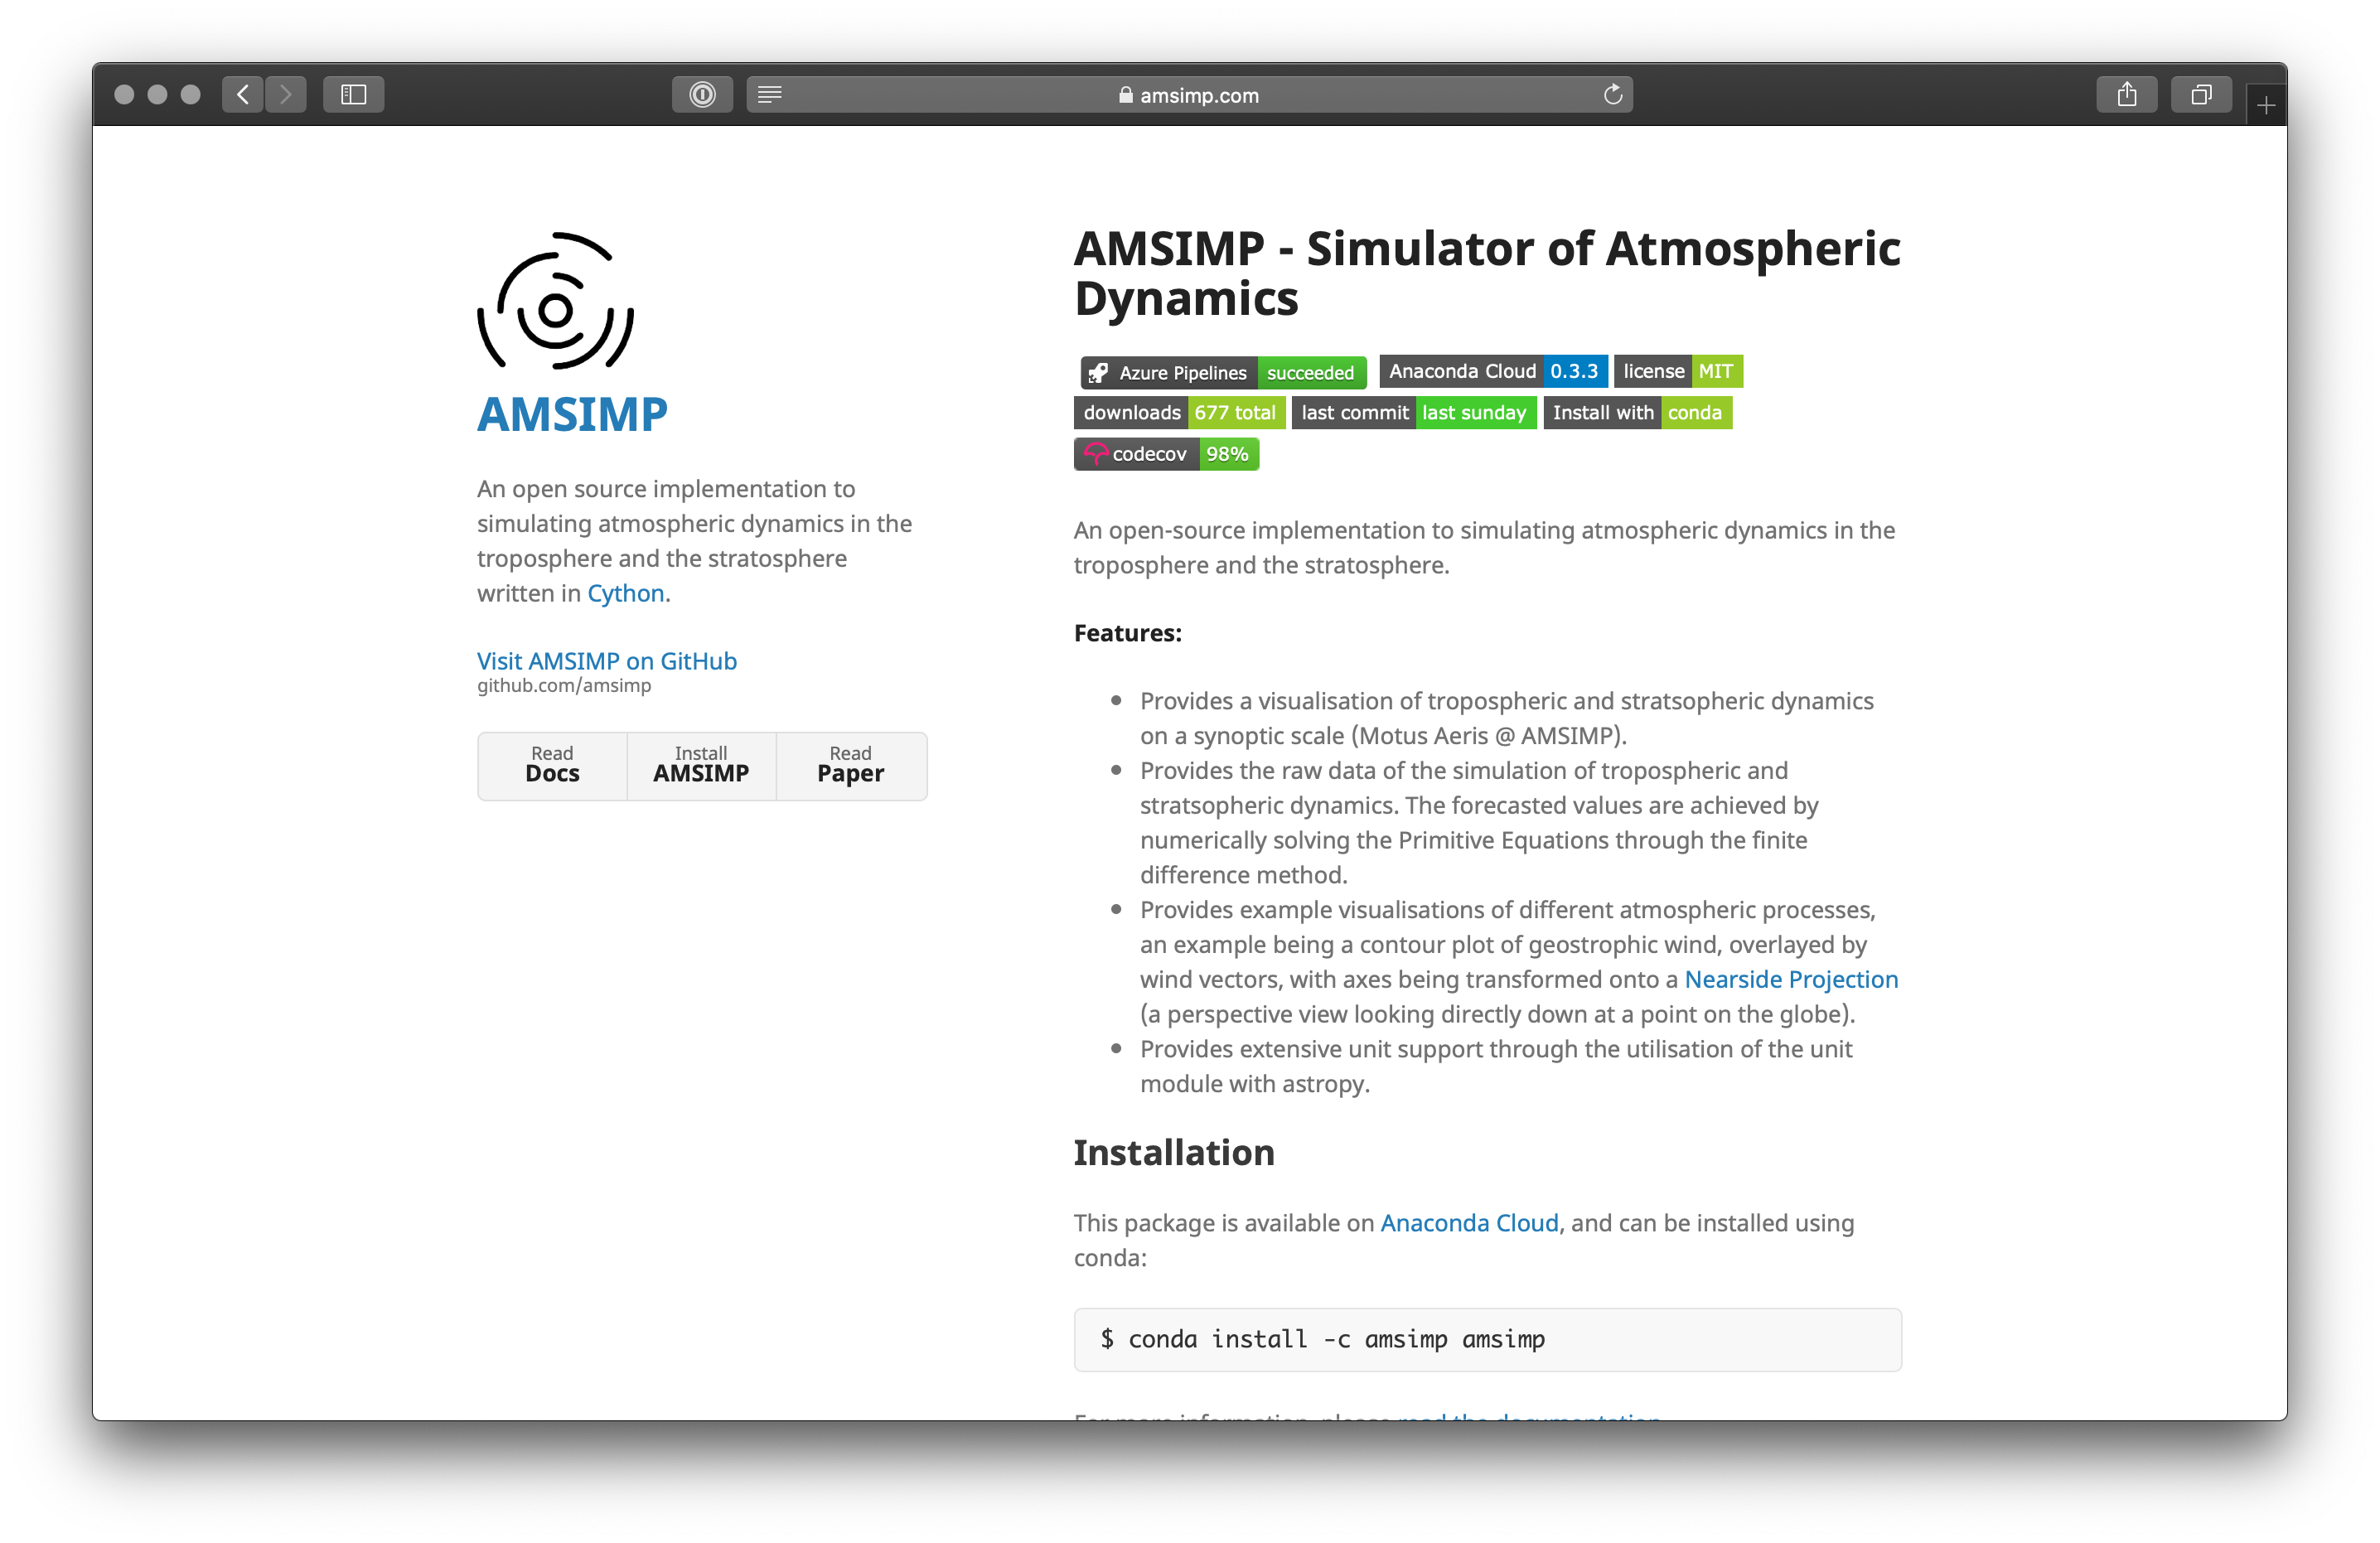
\includegraphics[width=.8\linewidth]{Images/website}
    \caption{A screenshot of the website for the software.}
    \label{website}
\end{figure}

\section{Organisation of this Work}
The work contained in this project book is broken down into a number of different chapters:

\begin{itemize}
    \item Chapter \ref{2} is the primary background research chapter and provides all the necessary information to understand the equations that underline the software.
    \item Chapter \ref{3} outlines how the Primitive Equations (the Forecast Equations) and other related equations are utilised in the software.
    \item Chapter \ref{4} discusses some of the decisions made on the software development side of the project, such as, choosing an appropriate programming language for the task. 
    \item Chapter \ref{5} outlines a series of software benchmarking experiments to be carried out on the software.
    \item Chapter \ref{6} contains the results of the benchmarking described in the previous chapter.
    \item Chapter \ref{7} reviews the results and outcomes of the project, discusses the limitations of the software, and lays out a road-map for the continued development and enhancement of the software. 
\end{itemize}

\section{Background Research}
This project (and by extension, the software), focuses on simulating atmospheric dynamics using the finite difference scheme. In this model, the globe is divided into cells. You can imagine this as cutting the atmosphere up into cuboids of air of equal volume. The software then solves the relevant equation for the given atmospheric parameter that is required at the middle of the cuboid. After which point, this value is used as an approximation for the entire cuboid. 

\hfill

\begin{center}
    \begin{tikzpicture}[every edge quotes/.append style={auto, text=black}]
        \pgfmathsetmacro{\cubex}{2}
        \pgfmathsetmacro{\cubey}{1}
        \pgfmathsetmacro{\cubez}{1.5}
        \draw [draw=black, every edge/.append style={draw=black, densely dashed, opacity=.5}]
        (0,0,0) coordinate (o) -- ++(-\cubex,0,0) coordinate (a) -- ++(0,-\cubey,0) coordinate (b) edge coordinate [pos=1] (g) ++(0,0,-\cubez)  -- ++(\cubex,0,0) coordinate (c) -- cycle
        (o) -- ++(0,0,-\cubez) coordinate (d) -- ++(0,-\cubey,0) coordinate (e) edge (g) -- (c) -- cycle
        (o) -- (a) -- ++(0,0,-\cubez) coordinate (f) edge (g) -- (d) -- cycle;
        \path [every edge/.append style={draw=black, |-|}]
        (b) +(0,-5pt) coordinate (b1) edge ["$\Delta \lambda$"'] (b1 -| c)
        (b) +(-5pt,0) coordinate (b2) edge ["$\Delta z$"] (b2 |- a)
        (c) +(3.5pt,-3.5pt) coordinate (c2) edge ["$\Delta \phi$"'] ([xshift=3.5pt,yshift=-3.5pt]e);
    \end{tikzpicture}
\end{center}

Considering computers cannot do calculus, but can only carry out simple arithmetic operations, the finite difference method (the central difference scheme) is used to solve any partial differential equations (PDEs) that are utilised within the software. As such, spatial derivatives are replaced as follows:

\begin{equation}
    \frac{\partial f}{\partial x} \rightarrow \frac{f(x + \Delta x) - f(x - \Delta x)}{2 \Delta x}
\end{equation}

and similarly for time derivatives: 

\begin{equation}
    \frac{\partial Q}{\partial t} \rightarrow \frac{Q^{n+1} - Q^{n-1}}{2 \Delta t} = F^{n}
\end{equation}

Solving for $Q^{n+1}$, this can be written as:

\begin{equation}
    Q^{n+1} = Q^{n-1} + 2 \Delta t F^{n}
\end{equation}

By continuously repeating the calculations at a given point, one may acquire a forecast of any length for the specified atmospheric parameter\cite{nwp}.

It is also important to note that the wind velocities are assumed to be geostrophic. This is known as the geostrophic approximation, and is a result of geostrophic balance. Geostrophic balance is a condition which states that there is an exact balance between the Coriolis force, and the pressure gradient force in the atmosphere. This condition arises from the fact that the Rossby number at synoptic scales (on a large scale) being rather small, implying that the wind velocities are nearly geostrophic\cite{UiO}. This is discussed at greater depth in chapter \ref{3}. Fundamentally, however, this restricts the software to solely simulating atmospheric dynamics at a synoptic scale.

In regards to other possible open source implementations to simulating atmospheric dynamics, there is (to the author's knowledge), no software currently available to this effect.